
\chapter{Search for Spatially-extended \Acs{LAT} Sources}

\paperref{
  This chapter is based the second part of the the paper
  ``Search for Spatially Extended Fermi-LAT Sources Using Two Years of Data''
  by Lande et at al. 2012 ApJ, 756, 5}

  Following the work in \chapref{extended_analysis},
  we next test all sources
  in the second \fermi-LAT catalog (2FGL) for extension.
  We report the detection of seven new spatially extended sources.

\section{Analysis of Extended Sources Identified in the 2FGL Catalog}
\seclabel{validate_known}

As further validation of our method for studying
spatially extended sources, we reanalyzed the twelve spatially extended
sources which were included in the 2FGL catalog \citep{nolan_2012_fermi-large}.  
Even though these sources had all been the subjects of dedicated
analyses and separate publications, and had been fit with a variety
of spatial models,
it is valuable to show that
these sources are significantly extended using our systematic 
method assuming radially-symmetric uniform disk spatial models.  On the other hand, for some of
these sources a uniform disk spatial model does not well describe the
observed extended emission and so the dedicated 
publications by the LAT collaboration provide better models of these sources.

Six extended SNRs were
included in the 2FGL catalog: W51C, IC~443, W28, W44, the Cygnus Loop,
and W30
\citep{abdo_2009a_fermi-discovery,abdo_2010a_observation-supernova,abdo_2010d_fermi-large,abdo_2010a_gamma-ray-emission,katagiri_2011a_fermi-large,ajello_2012a_fermi-large}.
Using photons
with energies between
1 \gev and 100 \gev, our analysis significantly detected
that these six SNRs are spatially extended.

Two nearby satellite galaxies of the Milky Way the Large Magellanic Cloud (LMC)
and the Small Magellanic
Cloud (SMC) were included in the 2FGL catalog as spatially extended sources \citep{abdo_2010a_observations-large,abdo_2010a_detection-small}.  
Their extensions were significantly
detected using photons with energies between
1 \gev and 100 \gev. Our
fit extensions are comparable to the published result, but we note that
the previous LAT Collaboration publication on the LMC used a more complicated two 2D Gaussian surface
brightness profile when fitting it \citep{abdo_2010a_observations-large}.

Three PWNe, MSH\,15$-$52, Vela X, and HESS\,J1825$-$137, were fit as
extended sources in the 2FGL analysis \citep{abdo_2010a_detection-energetic,abdo_2010c_fermi-large,grondin_2011_detection-pulsar}.  
In the present analysis, HESS\,J1825$-$137
was significantly detected using photons with energies between 10
\gev and 100 \gev.  To avoid confusion with the nearby bright pulsar
PSR\,J1509$-$5850, MSH\,15$-$52 had to be analyzed at high energies.
Using photons with energies above 10 \gev, we fit the extension of
MSH\,15$-$52 to be consistent with the published size but with \tsext=6.6.

Our analysis was unable to resolve Vela X which would have required first
removing the pulsed photons from the Vela pulsar which was beyond the
scope of this paper.  Our analysis also failed to detect a significant
extension for the Centaurus A Lobes because
the shape of the source is significantly different from a uniform
radially-symmetric disk\citep{abdo_2010a_fermi-gamma-ray}.

Our analysis of these sources is summarized in
\tabref{known_extended_sources}.  This table includes the best fit
positions and extensions of these sources when fitting them 
with a radially-symmetric uniform disk model. It also
includes the best fit spectral parameters for each source.  The positions
and extensions of Vela X and the Centaurus A Lobes were taken from
\cite{abdo_2010c_fermi-large,abdo_2010a_fermi-gamma-ray} and are included in this table for completeness.

\section{Systematic Errors on Extension}
\seclabel{systematic_errors_on_extension}

We developed two criteria for estimating systematic errors
on the extensions of the sources.
First, we estimated a systematic error due to
uncertainty in our knowledge of the LAT PSF.  
Before launch, the LAT PSF
was determined by detector simulations which were verified in accelerator
beam tests \citep{atwood_2009a_large-telescope}. However, in-flight data revealed
a discrepancy above 3 \gev in the PSF compared to the angular
distribution of photons from bright AGN \citep{ackermann_2012a_fermi-large}.
Subsequently, the PSF was fit empirically to bright AGN and this
empirical parameterization is used in the P7\_V6 IRFs.  To account for
the uncertainty in our knowledge of the PSF, we refit our extended source
candidates using the pre-flight Monte Carlo representation of the PSF
and consider the difference in extension found using the two PSFs as a
systematic error on the extension of a source.  The same approach was used
in \cite{abdo_2010a_observation-supernova}.  We believe that our parameterization
of the PSF from bright AGN is substantially better than the Monte Carlo
representation of the PSF so this systematic error is conservative.

We estimated a second systematic error on the extension of a source
due to uncertainty in our model of the Galactic diffuse emission by
using an alternative 
approach to modeling the diffuse emission
which takes as input templates
calculated by
GALPROP\footnote{GALPROP is a software package for calculating the
Galactic $\gamma$-ray emission based on a model of cosmic-ray propagation
in the Galaxy and maps of the distributions of the 
components of the interstellar medium \citep{strong_1998a_propagation-cosmic-ray,vladimirov_2011a_galprop-webrun:}. 
See also \url{http://galprop.stanford.edu/} for details.} 
but then fits each template locally in
the surrounding region.
The particular GALPROP model that was used as input is described in
the analysis of the isotropic diffuse
emission with LAT data \citep{abdo_2010a_spectrum-isotropic}.  
The intensities of various components
of the Galactic diffuse emission were fitted individually using a
spatial distribution predicted by
the model.  
We considered separate contributions from
cosmic-ray interactions with the
molecular hydrogen, the atomic and ionized hydrogen, residual gas traced
by dust \citep{grenier_2005a_unveiling-extensive}, and the interstellar radiation
field. We further split the contributions from interactions with molecular
and atomic hydrogen to the Galactic diffuse emission according to the
distance from the Galactic center in which they are produced. Hence, we
replaced the standard diffuse emission model by 18 individually fitted
templates to describe individual components of the diffuse emission.
A similar crosscheck was used in an analysis of RX\,J1713.7$-$3946 
by the LAT Collaboration \citep{abdo_2011a_observations-young}.

It is not expected that this diffuse model is superior to the standard
LAT model obtained through an all-sky fit.  However, adding degrees of
freedom to the background model can remove likely spurious sources that
correlate with features in the Galactic diffuse emission.  Therefore,
this tests systematics that may be due to imperfect modeling of the
diffuse emission in the region. 
Nevertheless, this alternative approach to modeling the diffuse emission
does not test all systematics related to the diffuse emission model. In
particular, because the alternative approach uses the same underlying gas
maps, it is unable to be used to assess systematics due to insufficient
resolution of the underlying maps. Structure in the diffuse emission that
is not correlated with these maps will also not be assessed by this test.

We do not expect the systematic error due to uncertainties in the PSF
to be correlated with the systematic error due to uncertainty in the
Galactic diffuse emission. Therefore, the total systematic error on the
extension of a source was obtained by adding the two errors in quadrature.

There is another systematic error on the size of a source due to issues
modeling nearby sources in crowded regions of the sky. It is beyond the
scope of this paper to address this systematic error. Therefore, 
for sources in crowded regions the systematic
errors quoted in this paper 
may not represent the full set of systematic errors associated with this analysis.

\section{Extended Source Search Method}
\seclabel{extended_source_search_method}


Having demonstrated that we understand the statistical
issues associated with analyzing spatially extended sources
(\subsecref{monte_carlo_validation} and \secref{test_2lac_sources}) and
that our method can correctly analyze the extended sources included in
2FGL (\secref{validate_known}), we applied this method to search for
new spatially extended \gev sources.
The data and general analysis setting is as described in \secref{test_2lac_sources}.

Ideally, we would apply a completely blind and uniform search that
tests the extension of each 2FGL source in the presence of all other
2FGL sources to find a complete list of all spatially extended sources.
As our test of AGN in \secref{test_2lac_sources} showed, at high
Galactic latitude where the source density is not as large and the
diffuse emission is less structured, this method works well.

But this is infeasible in the Galactic plane where we 
are most likely to discover new spatially extended sources.  In the Galactic plane,
this analysis is challenged by our imperfect model of the diffuse
emission and by an imperfect model of nearby sources.  The Monte Carlo
study in \secref{dual_localization_method}
showed that the overall likelihood would greatly increase by fitting
a spatially extended source as two point-like sources so we expect
that spatially extended sources would be modeled in the 2FGL catalog as
multiple point-like sources. Furthermore, the positions of other nearby sources
in the region close to an extended source could be biased by not correctly
modeling the extension of the source.  The 2FGL catalog contains a
list of sources significant at energies above 100 \mev whereas we are
most sensitive to spatial extension at higher energies.
We therefore expect that at higher energies our analysis would be complicated
by 2FGL sources no longer significant and by 2FGL
sources whose positions were biased by diffuse emission at lower energies.

To account for these issues, we first produced a large list of possibly
extended sources employing very liberal search criteria and then
refined the analysis of the promising candidates on a case by case basis.
Our strategy was to test all point-like 2FGL sources for extension assuming
they had a uniform radially-symmetric disk spatial model
and a power-law spectral model.  Although not all extended sources are
expected to have a shape very similar to a uniform disk, \subsecref{compare_source_size} showed that for many spatially
extended sources the wide PSF of the LAT and limited statistics makes
this a reasonable approximation.  On the other hand, choosing this
spatial model biases us against finding extended sources that are not
well described by a uniform disk model such as shell-type SNRs.

Before testing for extension, we automatically removed from the background
model all other 2FGL sources within 0\fdg5 of the source.  This distance
is somewhat arbitrary, but was picked in hopes of finding extended
sources with sizes on the order of $\sim1\degree$ or smaller. On the
other hand, by removing these nearby background sources we expect to
also incorrectly add to our list of extended source candidates
point-like sources that
are confused with nearby sources.  To screen out obvious cases of source
confusion, we performed the dual localization procedure described in
\secref{dual_localization_method} to compare the extended source
hypothesis to the hypothesis of two independent point-like sources.

As was shown in \subsecref{extension_sensitivity}, little sensitivity is gained by
using photons with energies below 1 \gev. In addition,
the broad PSF at low energy makes the analysis more susceptible to systematic
errors arising from source confusion due to nearby soft point-like sources
and by uncertainties in our modeling of the Galactic diffuse emission. 
For these reasons,
we performed our search using only photons with energies between 1 \gev
and 100 \gev.

We also performed a second search for extended sources using only
photons with energies between 10 \gev and 100 \gev.  Although this
approach tests the same sources, it is complementary because the Galactic
diffuse emission is even less dominant above 10 \gev and because source
confusion is less of an issue.  A similar procedure was used to detect
the spatial extensions of MSH\,15$-$52 and
HESS\,J1825$-$137 with the LAT \citep{abdo_2010a_detection-energetic,grondin_2011_detection-pulsar}.

When we applied this test to the 1861 point-like sources in the 2FGL catalog, our
search found 117 extended source candidates in the 1 \gev to 100 \gev
energy range and 11 extended source candidates in the 10 \gev to 100
\gev energy range. Most of the extended sources found above 10 \gev were
also found above 1 \gev and in many cases multiple nearby point-like
sources were found to be extended even though they fit the same emission region.
For example, the sources 2FGL\,J1630.2$-$4752, 2FGL\,J1632.4$-$4753c 2FGL\,J1634.4$-$4743c,
and 2FGL\,J1636.3$-$4740c were all found to be spatially extended in the
10 \gev to 100 \gev energy range even though they all fit to similar
positions and sizes.  For these situations, we manually discarded all
but one of the 2FGL sources.

Similarly, many of these sources were confused with nearby
point-like sources or influenced by large-scale residuals in the
diffuse emission.  To help determine which of these fits found
truly extended sources and when the extension was
influenced by source confusion and diffuse emission, we generated a
series of diagnostic plots.  For each candidate, we generated a map
of the residual TS by adding a new point-like source of spectral index 2 into the
region at each position and finding the increase in likelihood when fitting
its flux. \figref{res_tsmaps} shows this map around the
most significantly extended source IC~443 when it is modeled both as a
point-like source and as an extended source.  The residual TS
map indicates
that the spatially extended model for IC~443 is a significantly better
description of the observed photons and that there is no $\ts>25$
residual in the region after modeling the source as being spatially extended.
We also generated plots of the sum of all counts within a given distance of
the source and compared them to the model predictions assuming the emission
originated from a point-like source.  An example radial integral plot
is shown for the extended source IC~443 in \figref{four_plots_ic443}.
For each source, we also made diffuse-emission-subtracted smoothed counts
maps (shown for IC~443 in \figref{four_plots_ic443}).

We found by visual inspection that in many
cases our results were strongly influenced by large-scale residuals in the
diffuse emission and hence the extension measure was unreliable.  This was
especially true in our analysis of sources in the 1 \gev to 100 \gev
energy range.  An example of such a case is 2FGL\,J1856.2+0450c analyzed
in the 1 \gev to 100 \gev energy range. \figref{example_bad_fit}
shows a diffuse-emission-subtracted smoothed counts map for
this source with the best
fit extension of the source overlaid. There appear to be large-scale
residuals in the diffuse emission in this region along the Galactic plane.
As a result, 2FGL\,J1856.2+0450c is fit to an extension of $\sim2\degree$
and the result is statistically significant with \tsext=45.4. However,
by looking at the residuals it is clear that this complicated region is
not well modeled. We manually discard sources like this.

We only selected extended source
candidates in regions that did not appear dominated by these issues and
where there was a multiwavelength
counterpart. Because of these systematic issues, this search can not be
expected to be complete and it is likely that there are other spatially
extended sources that this method missed.

For each candidate that was not biased by neighboring point-like
sources or by large-scale residuals in the diffuse emission model, we
improved the model of the region by deciding on a case by case basis which
background point-like sources should be kept.  We kept in our model the
sources that we
believed represented physically distinct sources and we removed 
sources that we believed were included in the 2FGL catalog to compensate
for residuals induced by not modeling the extension of the source.
Soft nearby point-like 2FGL sources that were not significant at higher energies
were frozen to the spectras predicted by 2FGL.
When deciding
which background sources to keep and which to remove, we used 
multiwavelength information about possibly extended source counterparts
to help guide our choice. For each extended source presented in 
\secref{new_ext_srcs_section}, we describe any modifications from 2FGL
of the background model that were performed.
In \tabref{fake_2fgl_sources}, we summarize the sources in
the 2FGL catalog that we have concluded here correspond to residuals
induced by not modeling the extensions of nearby extended sources.

The best fit positions of nearby point-like sources can be influenced by
the extended source and vice versa.  Similarly,
the best fit positions of nearby point-like sources in the 2FGL catalog can be biased
by systematic issues at lower energies.
Therefore, after selecting the list of background sources, we iteratively
refit the positions and spectra of nearby background sources as well as
the positions and extensions of the analyzed spatially extended
sources until the overall fit converged globally.  For each extended
source, we will describe the positions of any relocalized background
sources.

After obtaining the overall best fit positions and extensions of all
of the sources in the region using \pointlike, we refit the spectral
parameters of the region using \gtlike.  With \gtlike, we obtained a
second measure of \tsext.  We only consider a source to be extended when
both \pointlike and \gtlike agree that $\tsext\ge16$. 
We further required that $\tsext\ge16$ using the 
alternative approach to modeling the diffuse emission
presented in \secref{systematic_errors_on_extension}.
We then replaced the spatially extended source with two point-like
sources and refit the positions and spectra of the
two point-like sources to calculate \tsinc.
We only consider a source to be spatially extended, instead of being
the result of confusion of two point-like sources, if $\tsext>\tsinc$.
As was shown in \secref{dual_localization_method}, this test is
fairly powerful at removing situations in which the emission actually
originates from two distinct point-like sources instead of one spatially
extended source.  On the other hand, it is still possible that longer
observations could resolve additional structure or new sources 
that the analysis cannot currently detect. 
Considering the very complicated morphologies
of extended sources observed at other wavelengths and the high density
of possible sources that are expected to emit at \gev energies, it is
likely that in some of these regions further observations will reveal
that the emission is significantly more complicated than the simple
radially-symmetric uniform disk model that we assume.



\section{New Extended Sources}
\seclabel{new_ext_srcs_section}

Nine extended sources not included in the 2FGL catalog were found by our
extended source search. Two of these have been previously
studied in dedicated publications: RX\,J1713.7$-$3946 and Vela
Jr. \citep{abdo_2011a_observations-young,tanaka_2011a_gamma-ray-observations}.
Two of these sources were
found when using photons with energies between 1 \gev and 100 \gev and seven
were found when using photons with energies between 10 \gev and 100 \gev.
For the sources found at energies above 10 \gev, we restrict our
analysis to higher energies because of the issues
of source confusion and diffuse emission modeling described in
\secref{extended_source_search_method}.
The spectral and spatial properties of these nine sources are summarized
in \tabref{new_ext_srcs_table} and the results of our investigation of
systematic errors are presented in \tabref{alt_diff_model_results}.
\tabref{alt_diff_model_results}
also
compares the likelihood assuming the source is spatially
extended to the likelihood assuming 
that the emission originates from two independent point-like
sources. For these new extended sources, $\tsext>\tsinc$ 
so we conclude that 
the \gev emission does not originate from two physically
distinct point-like sources (see \secref{dual_localization_method}).  
\tabref{alt_diff_model_results} also includes the
results of the extension fits using variations of the PSF and the Galactic
diffuse model described in \secref{systematic_errors_on_extension}.
There is good agreement between \tsext and the fit size using the standard
analysis, the alternative approach to modeling the diffuse emission, and the alternative PSF.
This suggests that the sources are robust against mis-modeled features in the diffuse
emission model and uncertainties in the PSF.

\subsection{2FGL\,J0823.0$-$4246}
\subseclabel{section_2FGL_J0823.0-4246}

2FGL\,J0823.0$-$4246 was found by our search to be an extended source
candidate in the 1 \gev to 100 \gev energy range and is spatially
coincident with the SNR Puppis A.  \figref{1FGL_J0823.3-4248} shows
a counts map of this source. There are two nearby 2FGL sources 2FGL\,J0823.4$-$4305
and 2FGL\,J0821.0$-$4254 that are also coincident with the SNR but that
do not appear to represent physically distinct sources.
We conclude that
these nearby point-like sources
were included in the 2FGL catalog to compensate for residuals induced
by not modeling the extension of this source and
removed them from our model of the sky.
After removing these sources, 2FGL\,J0823.0$-$4246 was found to have an extension 
$\sigma=0\fdg37\pm0\fdg03_\stat\pm0\fdg02_\sys$ with 
$\tsext=48.0$.  \figref{snr_seds} shows the spectrum of
this source.

Puppis A has been studied in detail in radio \citep{castelletti_2006a_observations-puppis}, 
and  X-ray \citep{petre_1996a_central-stellar,hwang_2008a_x-ray-emitting-ejecta}.
The fit extension of 2FGL\,J0823.0$-$4246
matches well the size of Puppis A in X-ray.  The distance of Puppis A was
estimated at 2.2 kpc \citep{reynoso_1995a_observations-neutral,reynoso_2003a_observations-neutral} and leads to a 1
\gev to 100 \gev luminosity of $\sim 3\times 10^{34}$ ergs$\,\second^{-1}$.
No molecular clouds have been observed directly adjacent to Puppis A
\citep{paron_2008a_high-resolution-observations}, similar to the LAT-detected Cygnus Loop SNR
\citep{katagiri_2011a_fermi-large}.  The luminosity of Puppis A is also smaller
than that of other SNRs believed to interact with molecular clouds
\citep{abdo_2009a_fermi-discovery,abdo_2010a_observation-supernova,abdo_2010a_gamma-ray-emission,abdo_2010d_fermi-large,abdo_2010a_fermi-lat-study}.

\subsection{2FGL\,J0851.7$-$4635}
\subseclabel{section_2FGL_J0851.7-4635}

2FGL\,J0851.7$-$4635 was found by our search to be an extended source
candidate in the 10 \gev to 100 \gev energy range and is spatially
coincident with the SNR Vela Jr. This source was recently studied by the LAT
Collaboration in \cite{tanaka_2011a_gamma-ray-observations}.  \figref{Vela_Jr} shows a counts
map of the source.  Overlaid on \figref{Vela_Jr} are \tev
contours of Vela Jr. \citep{aharonian_2007a_h.e.s.s.-observations}.
There are three
point-like 2FGL sources 2FGL\,J0848.5$-$4535,
2FGL\,J0853.5$-$4711, and
2FGL\,J0855.4$-$4625
which correlate with the 
multiwavelength
emission of
this SNR but do not appear to be physically distinct sources.
They were most likely included in the 2FGL catalog to compensate for residuals
induced by not modeling the extension of Vela Jr. and were removed
from our model of the sky.  

With this model of the background, 2FGL\,J0851.7$-$4635 was found to
have an extension of $\sigma=1\fdg15\pm0\fdg08_\stat\pm0\fdg02_\sys$ with
$\tsext=86.8$.  The LAT size matches
well the \tev morphology of Vela Jr.  While fitting the extension
of 2FGL\,J0851.7$-$4635, we iteratively relocalized the position
of the nearby point-like 2FGL source 2FGL\,J0854.7$-$4501 to
$(l,b)=(266\fdg24,0\fdg49)$ to better fit its position at high energies.
    



\subsection{2FGL\,J1615.0$-$5051}
\subseclabel{section_2FGL_J1615.0-5051}

2FGL\,J1615.0$-$5051 and 2FGL\,J1615.2$-$5138 were both found to be
extended source candidates in the 10 \gev to 100 \gev energy range. Because
they are less than $1\degree$ away from each other, they needed to be analyzed
simultaneously.  2FGL\,J1615.0$-$5051 is spatially coincident with
the extended \tev source HESS\,J1616$-$508 and 2FGL\,J1615.2$-$5138
is coincident with the extended \tev source HESS\,J1614$-$518.
\figref{1FGL_J1613.6-5100c} shows a counts map of these sources and
overlays the \tev contours of HESS\,J1616$-$508 and HESS\,J1614$-$518
\citep{aharonian_2006_h.e.s.s.-survey}.  The figure shows that the 2FGL source
2FGL\,J1614.9$-$5212 is very close to 2FGL\,J1615.2$-$5138 and correlates
with the same extended \tev source as 2FGL\,J1615.2$-$5138.  We concluded
that this source was included in the 2FGL catalog to compensate for residuals induced
by not modeling the extension of 2FGL\,J1615.2$-$5138 and removed
it from our model of the sky.  

With this model of the sky, we iteratively fit the extensions of
2FGL\,J1615.0$-$5051 and 2FGL\,J1615.2$-$5138.
2FGL\,J1615.0$-$5051 was found to have an extension 
$\sigma=0\fdg32\pm0\fdg04_\stat\pm0\fdg01_\sys$ and
\tsext=16.7.


The \tev counterpart of 2FGL\,J1615.0$-$5051 was fit
with a radially-symmetric Gaussian surface brightness profile with
$\sigma=0\fdg136\pm0\fdg008$ \citep{aharonian_2006_h.e.s.s.-survey}. This \tev size corresponds to a 68\%
containment radius of $\rsixeight=0\fdg21\pm0\fdg01$, comparable to the
LAT size $\rsixeight=0\fdg26\pm0\fdg03$.  \figref{hess_seds} shows
that the spectrum of 2FGL\,J1615.0$-$5051 at \gev energies connects to
the spectrum of HESS\,J1616$-$508 at \tev energies.

HESS\,J1616$-$508 is located in the region of two SNRs RCW103 (G332.4-04)
and Kes~32 (G332.4+0.1) but is not spatially coincident with either
of them \citep{aharonian_2006_h.e.s.s.-survey}.  HESS\,J1616$-$508 is near three
pulsars PSR\,J1614$-$5048, PSR\,J1616$-$5109, and PSR\,J1617$-$5055.
\citep{torii_1998a_discovery-millisecond,landi_2007a_j1616-508:-likely}.  Only
PSR\,J1617$-$5055 is energetically capable of powering the \tev emission
and \cite{aharonian_2006_h.e.s.s.-survey} speculated that HESS\,J1616$-$508 could
be a PWN powered by this young pulsar.  Because HESS\,J1616$-$508 is
$9\arcmin$ away from PSR\,J1617$-$5055, this would require an asymmetric
X-ray PWNe to power the \tev emission.  \chandra ACIS observations
revealed an underluminous PWN of size $\sim1\arcmin$ around the
pulsar that was not oriented towards the \tev emission, rendering this
association uncertain \citep{kargaltsev_2008a_young-energetic}.
No other promising counterparts were observed at X-ray and soft
$\gamma$-ray energies by \suzaku \citep{matsumoto_2007a_suzaku-observations}, \swiftxrt,
IBIS/ISGRBI, BeppoSAX and \xmmnewton \citep{landi_2007a_j1616-508:-likely}.
\cite{kargaltsev_2008a_young-energetic} discovered additional
diffuse emission towards the center of HESS\,J1616$-$508 using archival
radio and infared observations. Deeper observations will likely be
necessary to understand this $\gamma$-ray source.

\subsection{2FGL\,J1615.2$-$5138}
\subseclabel{section_2FGL_J1615.2-5138}

2FGL\,J1615.2$-$5138 was found
 to have an extension $\sigma=0\fdg42\pm0\fdg04_\stat\pm0.02_\sys$
with $\tsext=46.5$.
To test for the possibility that
2FGL\,J1615.2$-$5138 is not spatially extended but instead composed
of two point-like sources (one of them represented in the 2FGL catalog by
2FGL\,J1614.9$-$5212), we refit 2FGL\,J1615.2$-$5138 as two point-like
sources.  Because $\tsinc=35.1$ is less than $\tsext=46.5$, we conclude that
this emission does not originate from two closely-spaced point-like sources.

2FGL\,J1615.2$-$5138 is spatially coincident with 
the extended \tev source HESS\,J1614$-$518.
H.E.S.S. measured a 2D Gaussian extension of $\sigma=0\fdg23\pm0\fdg02$
and $\sigma=0\fdg15\pm0\fdg02$ in the semi-major and
semi-minor axis. This corresponds to a 68\% containment size of
$\rsixeight=0\fdg35\pm0\fdg03$ and $0\fdg23\pm0\fdg03$,  consistent with
the LAT size $\rsixeight=0\fdg34\pm0\fdg03$.  \figref{hess_seds}
shows that the spectrum of 2FGL\,J1615.2$-$5138 at \gev energies connects
to the spectrum of HESS\,J1614$-$518 at \tev energies.  Further data
collected by H.E.S.S. in 2007 resolve a double peaked structure at
\tev energies but no spectral variation across this source, suggesting
that the emission is not the confusion of physically separate sources
\citep{rowell_2008a_closer-unidentified}.  This double peaked structure is
also hinted at in the LAT counts map in \figref{1FGL_J1613.6-5100c}
but is not very significant.  The \tev source was also detected by
CANGAROO-III \citep{mizukami_2011a_cangaroo-iii-observation}.

There are five nearby pulsars, but none are luminous enough to
provide the energy output required to power the $\gamma$-ray
emission \citep{rowell_2008a_closer-unidentified}.  HESS\,J1614$-$518
is spatially coincident with a young open cluster Pismis 22
\citep{landi_2007a_j1614-518:-detection,rowell_2008a_closer-unidentified}.  \suzaku detected
two promising X-ray candidates. Source A is an extended source consistent
with the peak of HESS\,J1614$-$518 and source B coincident with Pismis 22
and towards the center but in a relatively dim region of HESS\,J1614$-$518
\citep{matsumoto_2008a_discovery-extended}.  Three hypotheses have been presented to
explain this emission: either source A is an SNR powering the $\gamma$-ray
emission; source A is a PWN powered by an undiscovered pulsar in either
source A or B; and finally that the emission may arise from hadronic
acceleration in the stellar winds of Pismis 22 \citep{mizukami_2011a_cangaroo-iii-observation}.

\subsection{2FGL\,J1627.0$-$2425c}
\subseclabel{section_2FGL_J1627.0-2425c}

2FGL\,J1627.0$-$2425c was found by our search to
have an extension $\sigma=0\fdg42\pm0\fdg05_\stat\pm0\fdg16_\sys$ with
$\tsext=32.4$
using photons with energies between 1 \gev and 100 \gev.  
\figref{1FGL_J1628.6-2419c} shows a counts map of this source.

This source is in a region of remarkably complicated diffuse emission.
Even though it is $16\degree$ from the Galactic plane, this source is on
top of the core of the Ophiuchus molecular cloud which contains massive
star-forming regions that are bright in infrared.  The region also has
abundant molecular and atomic gas traced by CO and H~I and significant 
dark gas found only by its association with dust emission
\citep{grenier_2005a_unveiling-extensive}. Embedded star-forming regions make it even
more challenging to measure the column density of dust.  Infared and 
CO ($J=1\rightarrow 0$)
contours are overlaid on \figref{1FGL_J1628.6-2419c} and show good
spatial correlation with the \gev emission \citep{young_1986a_high-resolution-observations,de-geus_1990a_survey-clouds}.
This source might 
represent $\gamma$-ray emission from the interactions of cosmic rays with
interstellar gas which has not been accounted for in the LAT diffuse
emission model.


\subsection{2FGL\,J1632.4$-$4753c}
\subseclabel{section_2FGL_J1632.4-4753c}

2FGL\,J1632.4$-$4753c was found by our search to be an extended source
candidate in the 10 \gev to 100 \gev energy range but is in a crowded
region of the sky.  It is spatially coincident with the \tev source
HESS\,J1632$-$478.  \figref{1FGL_J1632.9-4802c}a shows a counts
map of this source and overlays \tev contours of HESS\,J1632$-$478
\citep{aharonian_2006_h.e.s.s.-survey}.  There are six nearby point-like 2FGL
sources that appear to represent physically distinct sources
and were included in our background model: 2FGL\,J1630.2$-$4752, 2FGL\,J1631.7$-$4720c, 2FGL\,J1632.4$-$4820c, 2FGL\,J1635.4$-$4717c,
2FGL\,J1636.3$-$4740c, and
2FGL\,J1638.0$-$4703c. On the
other hand, one point-like 2FGL source 2FGL\,J1634.4$-$4743c  correlates
with the extended \tev source and at \gev energies does
not appear physically separate. 
It is very close to the position of 2FGL\,J1632.4$-$4753c
and does not show spatially separated emission in the observed photon distribution.
We therefore removed this source from our model of the
background.  \figref{1FGL_J1632.9-4802c}b shows the same region with
the background sources subtracted.  With this model, 2FGL\,J1632.4$-$4753c
was found to have an extension $\sigma=0\fdg35\pm0\fdg04_\stat\pm0\fdg02_\sys$
with $\tsext=26.9$.  While fitting the
extension of 2FGL\,J1632.4$-$4753c, we iteratively relocalized
2FGL\,J1635.4$-$4717c to $(l,b)=(337\fdg23,0\fdg35)$ and
2FGL\,J1636.3$-$4740c to $(l,b)=(336\fdg97,-0\fdg07)$.

H.E.S.S measured an extension of $\sigma=0\fdg21\pm0\fdg05$ and
$0\fdg06\pm0\fdg04$ along the semi-major and semi-minor axes when
fitting HESS\,J1632$-$478 with an elliptical 2D Gaussian surface
brightness profile.  This corresponds to a 68\% containment size
$\rsixeight=0\fdg31\pm0\fdg08$ and $0\fdg09\pm0\fdg06$ along
the semi-major and semi-minor axis, consistent with the LAT size
$\rsixeight=0\fdg29\pm0\fdg04$.  \figref{hess_seds} shows that
the spectrum of 2FGL\,J1632.4$-$4753c at \gev energies connects to the
spectrum of HESS\,J1632$-$478 at \tev energies.

\cite{aharonian_2006_h.e.s.s.-survey} argued that HESS\,J1632$-$478
is positionally coincident with the hard X-ray source
IGR\,J1632$-$4751 observed by \asca, INTEGRAL, and \xmmnewton
\citep{sugizaki_2001a_faint-x-ray,tomsick_2003a_j16320-4751,rodriguez_2003a_xmm-newton-observation},
but this source is suspected to be a Galactic X-Ray Binary so the
$\gamma$-ray extension disfavors the association.  Further observations
by \xmmnewton discovered point-like emission coincident with the peak
of the H.E.S.S. source surrounded by extended emission of size
$\sim32\arcsec\times15\arcsec$ \citep{balbo_2010a_j1632-478:-energetic}.
They found in archival MGPS-2 data a spatially coincident extended
radio source \citep{murphy_2007a_second-epoch} and argued for a single
synchrotron and inverse Compton process producing the radio, X-ray, and \tev emission,
likely due to a PWN.  The increased size at \tev energies compared
to X-ray energies has previously been observed in several aging PWNe
including HESS\,J1825$-$137 \citep{gaensler_2003a_xmm-newton-observations,aharonian_2006_energy-dependent},
HESS\,J1640$-$465 \citep{aharonian_2006_h.e.s.s.-survey,funk_2007a_xmm-newton-observations},
and Vela X \citep{markwardt_1995a_x-ray-pulsar,aharonian_2006a_first-detection} and can be explained by
different synchrotron cooling times for the electrons that produce X-rays
and $\gamma$-rays.


\subsection{2FGL\,J1712.4$-$3941}
\subseclabel{section_2FGL_J1712.4-3941}

2FGL\,J1712.4$-$3941 was found by our search to be spatially extended
using photons with energies between 1 \gev and 100 \gev.  This source
is spatially coincident with the SNR RX\,J1713.7$-$3946 and was
recently studied by the LAT Collaboration in \cite{abdo_2011a_observations-young}.
To avoid issues related to uncertainties in the nearby Galactic
diffuse emission at lower energy, we restricted our analysis only
to energies above 10 \gev.  \figref{2FGL_J1712.4-3941} shows a
smoothed counts map of the source. Above 10 \gev, the \gev emission
nicely correlates with the \tev contours of RX\,J1713.7$-$3946
\citep{aharonian_2007a_primary-particle} and 2FGL\,J1712.4$-$3941 fit to an extension 
$\sigma=0\fdg56\pm0\fdg04_\stat\pm0\fdg02_\sys$ with $\tsext=38.5$.

\subsection{2FGL\,J1837.3$-$0700c}
\subseclabel{section_2FGL_J1837.3-0700c}

2FGL\,J1837.3$-$0700c was found by our search to be an extended source
candidate in the 10 \gev to 100 \gev energy range and is spatially
coincident with the \tev source HESS\,J1837$-$069.  This source is
in a complicated region.  \figref{1FGL_J1837.5-0659c}a shows a
smoothed counts map of the region and overlays the \tev contours of
HESS\,J1837$-$069 \citep{aharonian_2006_h.e.s.s.-survey}.  There are two very nearby
point-like 2FGL sources, 2FGL\,J1836.8$-$0623c and 2FGL\,J1839.3$-$0558c,
that clearly represent distinct sources.  On the other hand, there is
another source 2FGL\,J1835.5$-$0649 located between the three sources that
appears to correlate with the \tev morphology of HESS\,J1837$-$069 but
at \gev energies
does not appear to represent a physically distinct source.  We concluded
that this source was included in the 2FGL catalog to compensate for residuals induced by
not modeling the extension of this source and removed it from our model
of the sky.  \figref{1FGL_J1837.5-0659c}b shows a
counts map of this region after subtracting these background sources.
After removing 2FGL\,J1835.5$-$0649,
we tested for
source confusion by fitting 
2FGL\,J1837.3$-$0700c
instead as two point-like sources.
Because $\tsinc=10.8$ is less than $\tsext=18.5$, we conclude that this emission
does not originate from two nearby point-like sources.

With this model, 2FGL\,J1837.3$-$0700c was found to have an
extension $\sigma=0\fdg33\pm0\fdg07_\stat\pm0\fdg05_\sys$.
While fitting the extension of 2FGL\,J1837.3$-$0700c,
we iteratively relocalized the two closest
background sources along with the extension of 2FGL\,J1837.3$-$0700c but
their positions did not significantly change.  2FGL\,J1834.7$-$0705c
moved to $(l,b)=(24\fdg77,0\fdg50)$, 2FGL\,J1836.8$-$0623c moved
to $(l,b)=(25\fdg57,0\fdg32)$. 

H.E.S.S. measured an extension of
$\sigma=0\fdg12\pm0\fdg02$ and $0\fdg05\pm0\fdg02$ 
of the coincident \tev source HESS\,J1837$-$069 
along the semi-major and semi-minor axis when fitting this source
with an elliptical 2D Gaussian surface brightness profile.  This corresponds
to a 68\% containment radius of $\rsixeight=0\fdg18\pm0\fdg03$ and
$0\fdg08\pm0\fdg03$ along the semi-major and semi-minor axis. The
size is not significantly different from the LAT 68\% containment
radius of $\rsixeight=0\fdg27\pm0\fdg07$ (less than $2\sigma$).
\figref{hess_seds} shows that the spectrum of 2FGL\,J1837.3$-$0700c
at \gev energies connects to the spectrum of HESS\,J1837$-$069 at \tev
energies.

HESS\,J1837$-$069 is coincident with the hard and steady X-ray source
AX\,J1838.0$-$0655 \citep{bamba_2003a_diffuse-x-ray}.  This source was discovered
by RXTE to be a pulsar (PSR J1838-0655) 
sufficiently luminous to power the \tev emission
and was resolved by \chandra to be a bright point-like source surrounded
by a $\sim2\arcmin$ nebula \citep{gotthelf_2008a_discovery-young}. The
$\gamma$-ray emission may be powered by this pulsar.  The hard spectral
index and spatial extension of 2FGL\,J1837.3$-$0700c disfavor a pulsar
origin of the LAT emission and suggest instead that the \gev and \tev
emission both originate from the pulsar's wind.  There is another
X-ray point-like source AX\,J1837.3$-$0652 near HESS\,J1837$-$069
\citep{bamba_2003a_diffuse-x-ray} that was also resolved into a point-like
and diffuse component \citep{gotthelf_2008a_discovery-young}.  Although no
pulsations have been detected from it, it could also be a pulsar powering
some of the $\gamma$-ray emission.


\subsection{2FGL\,J2021.5+4026}
\subseclabel{section_2FGL_J2021.5+4026}

The source 2FGL\,J2021.5+4026 is associated with the $\gamma$-Cygni SNR 
and has been speculated
to originate from the interaction of accelerated particles in the SNR
with dense molecular clouds \citep{pollock_1985a_probable-identification,gaisser_1998a_gamma-ray-production}. This
association was disfavored when the \gev emission from this source
was detected to be pulsed \citep[PSR\,J2021+4026,][]{abdo_2010a_first-fermi}.
This pulsar was also observed by AGILE \citep{chen_2011a_study-gamma-ray}.

Looking at the same region at energies above 10 \gev, the pulsar is
no longer significant but we instead found in our search an extended
source candidate.  \figref{1FGL_J2020.0+4049} shows a counts map
of this source and overlays radio contours of $\gamma$-Cygni from the
Canadian Galactic Plane Survey \citep{taylor_2003a_canadian-galactic}.
There is good spatial overlap between the SNR and the \gev emission.

There is a nearby source 2FGL\,J2019.1+4040 that correlates with the radio
emission of $\gamma$-Cygni and at \gev energies 
does not appear to represent a physically
distinct source.  We concluded that it was included in the 2FGL catalog to compensate
for residuals induced by not modeling the extension of $\gamma$-Cygni and
removed it from our model of the sky.  With this model, 2FGL\,J2021.5+4026
was found to have an extension $\sigma=0\fdg63\pm0\fdg05_\stat\pm0\fdg04_\sys$
with $\tsext=128.9$.  \figref{snr_seds}
shows its spectrum.  The inferred size of this source at \gev energies
well matches the radio size of $\gamma$-Cygni.  Milagro detected
a $4.2\sigma$ excess at energies $\sim 30$ \tev from this location
\citep{abdo_2009a_fermi/large-telescope,abdo_2009a_milagro-observations}.  VERITAS also detected an
extended source VER\,J2019+407 coincident with the SNR above 200 \gev
and suggested that the \tev emission could be a shock-cloud interaction
in $\gamma$-Cygni \citep{weinstein_2009a_veritas-survey}.


\section{Discussion}

\clearpage
  \begin{figure}
      \ifcolorfigure
      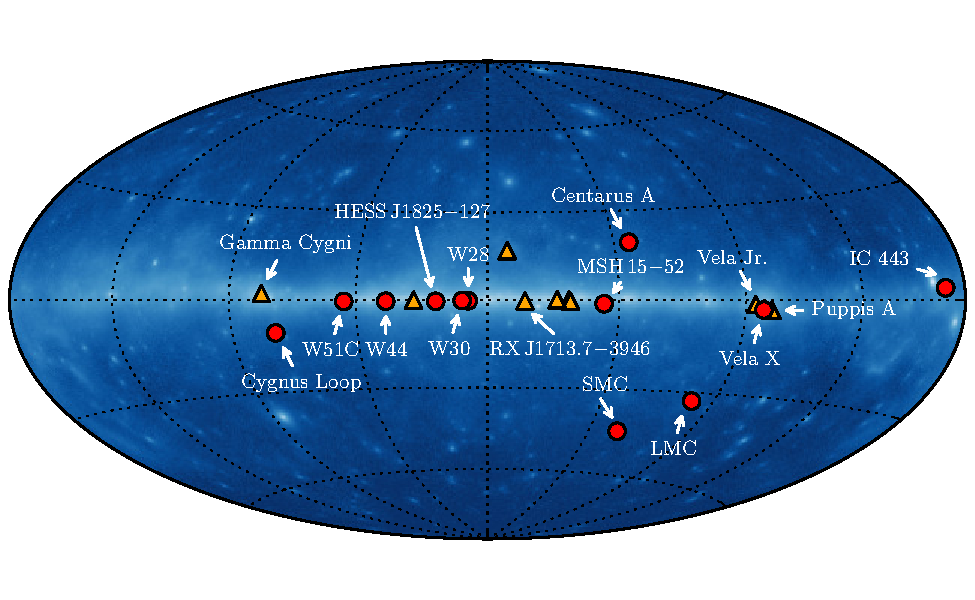
\includegraphics{summary_plots/allsky_extended_sources_color.pdf}
      \else
      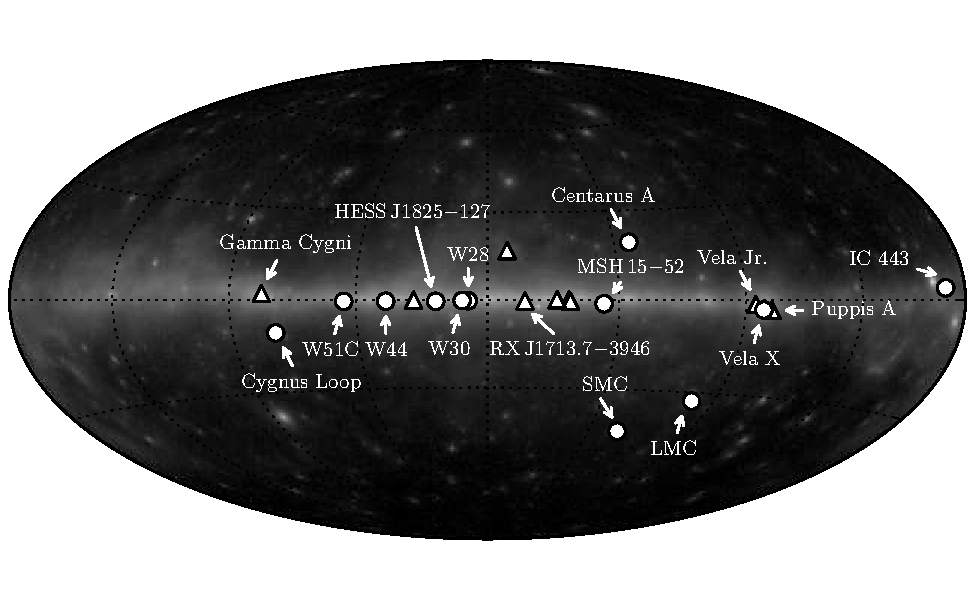
\includegraphics{summary_plots/allsky_extended_sources_bw.pdf}
      \fi
      % this plot came from /u/gl/lande/work/fermi/extended_catalog/2FGL/plots_for_paper/allsky/v2/run.py
      \caption{The 21
      spatially extended sources detected by the LAT
      at \gev energies 
      with 2 years of data.  The twelve extended sources included in
      2FGL are represented by the circular markers (colored red in the online
      version).  The nine new extended sources are represented by
      the triangular markers (colored orange).
      The source positions are overlaid on a 100 \mev to 100 \gev 
      Aitoff projection sky map of the LAT data in Galactic coordinates.
}
\figlabel{allsky_extended_sources}
  \end{figure}


Twelve extended sources were included in the 2FGL catalog and two additional extended
sources were studied in dedicated publications.  Using 2 years of
LAT data and a new analysis method, we presented the detection of seven
additional extended sources.  We also reanalyzed the spatial extents of the
twelve extended sources in the 2FGL catalog and the two additional sources.  The 21
extended LAT sources are located primarily along the Galactic plane
and their locations are shown in \figref{allsky_extended_sources}.
Most of the LAT-detected extended sources are expected to be of Galactic
origin as the distances of extragalactic sources (with the exception of
the local group Galaxies) are typically too large to be able to resolve
them at $\gamma$-ray energies.


\clearpage
\begin{figure}
    \ifcolorfigure
      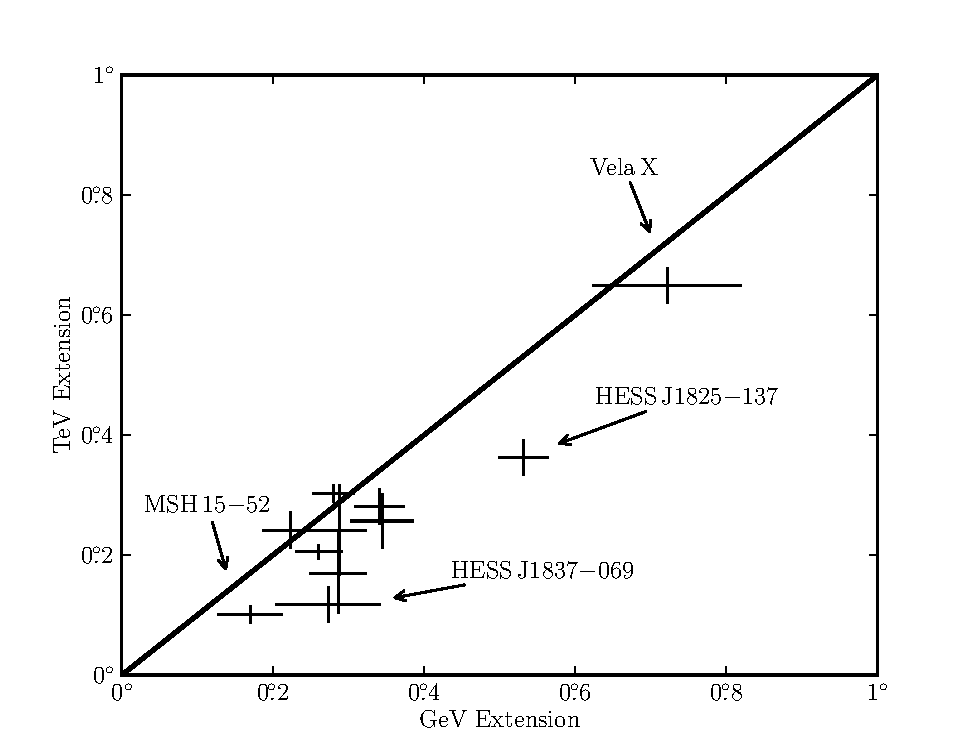
\includegraphics{summary_plots/gev_vs_tev_plot_color.pdf}
    \else
      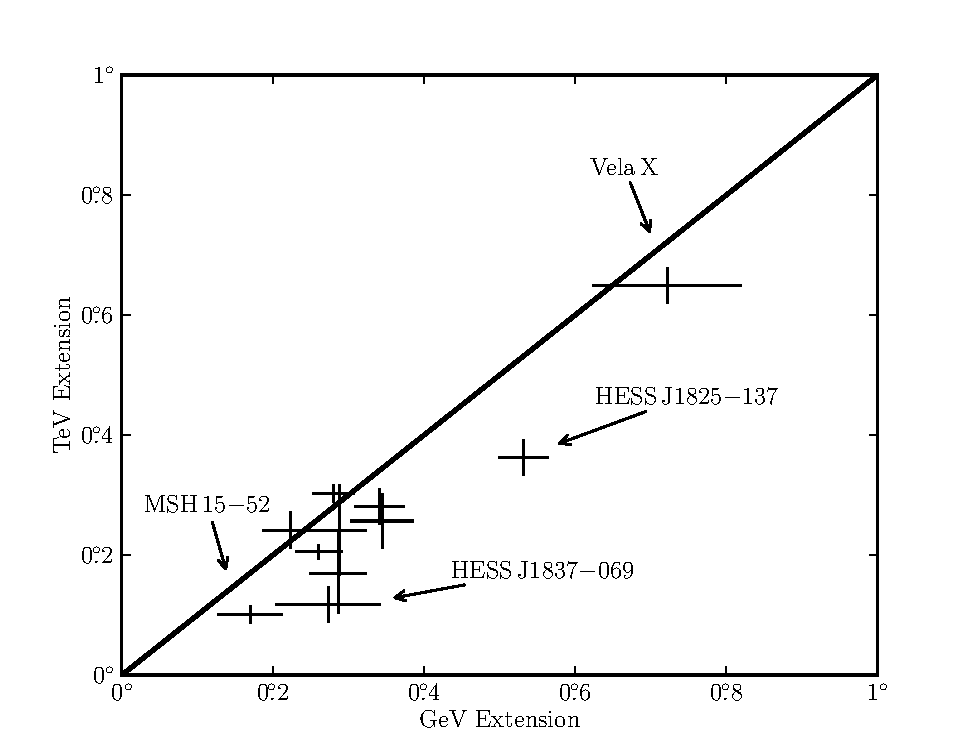
\includegraphics{summary_plots/gev_vs_tev_plot_bw.pdf}
      \fi
    % this plot came from /u/gl/lande/work/fermi/extended_catalog/2FGL/plots_for_paper/compare_tev_gev_sizes/v5/run.py
    \caption{
    A comparison of the sizes of extended sources detected at
    both \gev and \tev energies.  The \tev sizes of W30,
    2FGL\,J1837.3$-$0700c, 2FGL\,J1632.4$-$4753c, 2FGL\,J1615.0$-$5051,
    and 2FGL\,J1615.2$-$5138 are from \cite{aharonian_2006_h.e.s.s.-survey}.
    The \tev sizes of MSH\,15$-$52, HESS\,J1825$-$137,
    Vela X, Vela Jr., RX\,J1713.7$-$3946 and W28 are from
    \cite{aharonian_2005a_discovery-extended,aharonian_2006_energy-dependent,aharonian_2006a_first-detection,aharonian_2007a_h.e.s.s.-observations,aharonian_2007a_primary-particle,aharonian_2008a_discovery-energy}.
    The \tev size of IC~443 is from \cite{acciari_2009a_observation-extended} and
    W51C is from \cite{krause_2011a_probing-proton}.  The \tev
    sizes of MSH\,15$-$52, HESS\,J1614$-$518, HESS\,J1632$-$478, and
    HESS\,J1837$-$069 have only been reported with an elliptical 2D
    Gaussian fit and so the plotted sizes are the geometric 
    mean of the semi-major and semi-minor axis.
    The LAT extension of
    Vela X is from \cite{abdo_2010c_fermi-large}. 
    The \tev sources were fit assuming a 2D Gaussian surface brightness profile
    so the plotted \gev and \tev extensions were first converted to
    \rsixeight (see \subsecref{compare_source_size}).  
    Because of
    their large sizes, the shape of RX\,J1713.7$-$3946 and Vela Jr.
    were not directly fit at \tev energies and so are not included
    in this comparison. On the other hand, dedicated publications by the 
    LAT collaboration on
    these sources showed that their morphologies are consistent
    \citep{abdo_2011a_observations-young,tanaka_2011a_gamma-ray-observations}.
    The LAT
    extension errors are the statistical and systematic errors added
    in quadrature. 
}\figlabel{gev_vs_tev_plot}
  \end{figure}

For the LAT extended sources also seen at \tev energies,
\figref{gev_vs_tev_plot} shows that there is a good correlation
between the sizes of the sources at \gev and \tev energies. Even so,
the sizes of PWNe are expected to vary across the \gev and \tev energy
range and the size of HESS\,J1825$-$137 is significantly larger at
\gev than \tev energies \citep{grondin_2011_detection-pulsar}.  It is interesting
to compare the sizes of other PWN candidates at \gev and \tev energies,
but definitively measuring a difference in size would require a more in-depth analysis
of the LAT data using the same elliptical Gaussian spatial model.


\clearpage
\begin{figure}
    \ifcolorfigure
      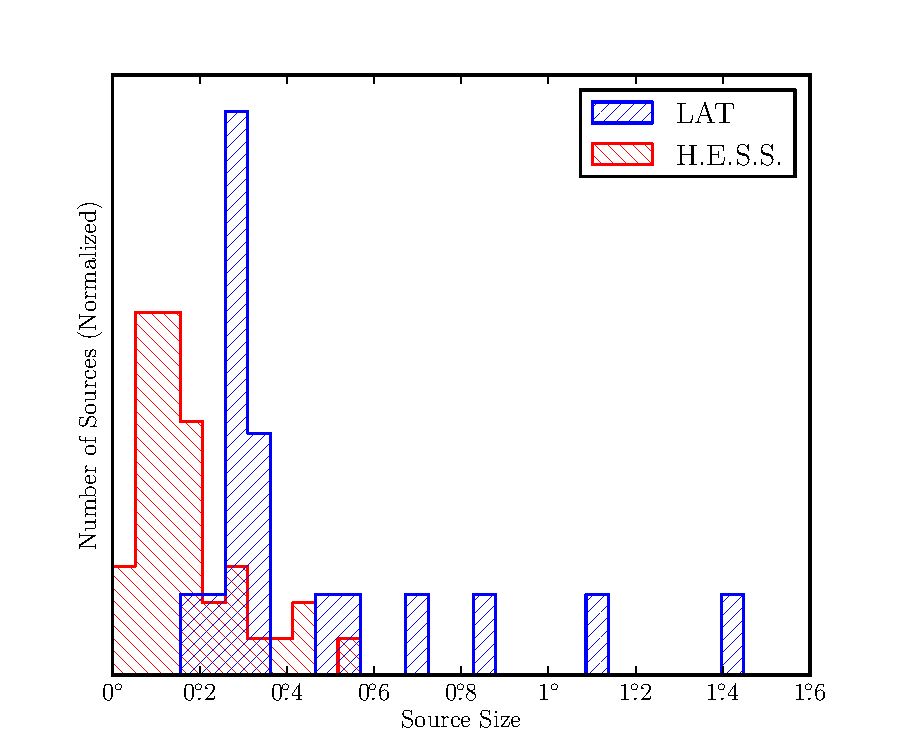
\includegraphics{summary_plots/gev_vs_tev_histogram_color.pdf}
    \else
      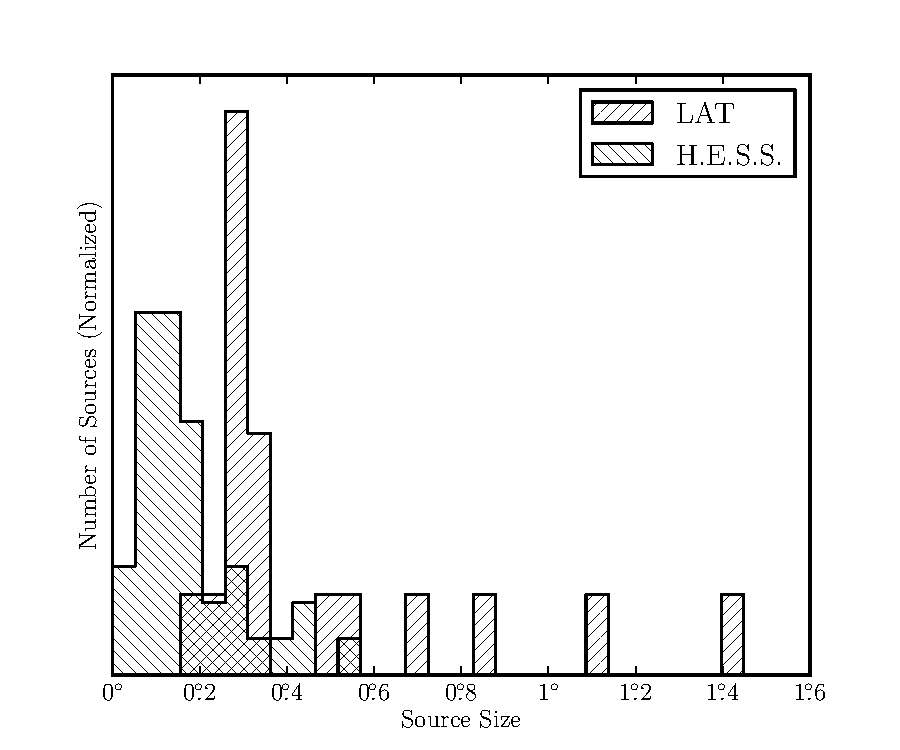
\includegraphics{summary_plots/gev_vs_tev_histogram_bw.pdf}
    \fi
    % this plot came from /u/gl/lande/work/fermi/extended_catalog/2FGL/plots_for_paper/extension_histogram/v5/extension_histogram.py
    \caption{
    The distributions of the sizes of 18 extended LAT sources
    at \gev energies
    (colored blue in the electronic version) and the sizes of the
    40 extended H.E.S.S. sources at \tev energies
    (colored red).  
    The H.E.S.S. sources were fit with a 2D Gaussian surface
    brightness profile so the LAT and H.E.S.S. sizes were first converted
    to \rsixeight. 
    The \gev size of Vela X is taken from \cite{abdo_2010c_fermi-large}.  
    Because of their large sizes, the shape of RX\,J1713.7$-$3946 and
    Vela Jr. were not directly fit at \tev energies
    and are not included in this comparison.
    Centaurus A is not included because of its large size.
    }\figlabel{gev_vs_tev_histogram}
  \end{figure}

\figref{gev_vs_tev_histogram} compares the sizes of the 21 extended
LAT sources to the 42 extended H.E.S.S. sources.\footnote{The 
\tev extension of
the 42 extended H.E.S.S. sources comes from the H.E.S.S. Source
Catalog \url{http://www.mpi-hd.mpg.de/hfm/HESS/pages/home/sources/}.}
Because of the large
field of view and all-sky coverage, the LAT can more easily measure
larger sources.  On the other hand, the 
better
angular resolution of air Cherenkov detectors allows them to measure a
population of extended sources below the resolution limit of the LAT (currently 
about $\sim0\fdg2$).  \fermi has a 5 year nominal mission lifetime with
a goal of 10 years of operation.  As \figref{time_sensitivity} shows,
the low background of the LAT at high energies allows its sensitivity 
to
these smaller sources to improve by a factor greater than the square root
of the relative exposures.  With increasing exposure, the LAT will likely begin to
detect and resolve some of these smaller \tev sources.

\clearpage
\begin{figure}
    \ifcolorfigure
      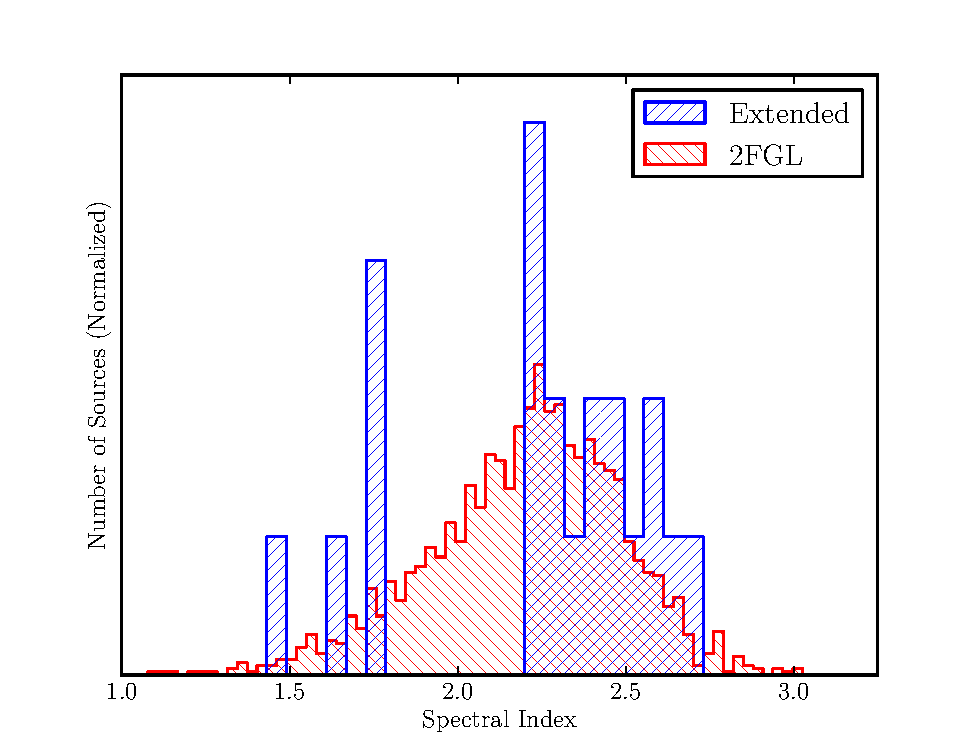
\includegraphics{summary_plots/compare_index_2FGL_color.pdf}
    \else
      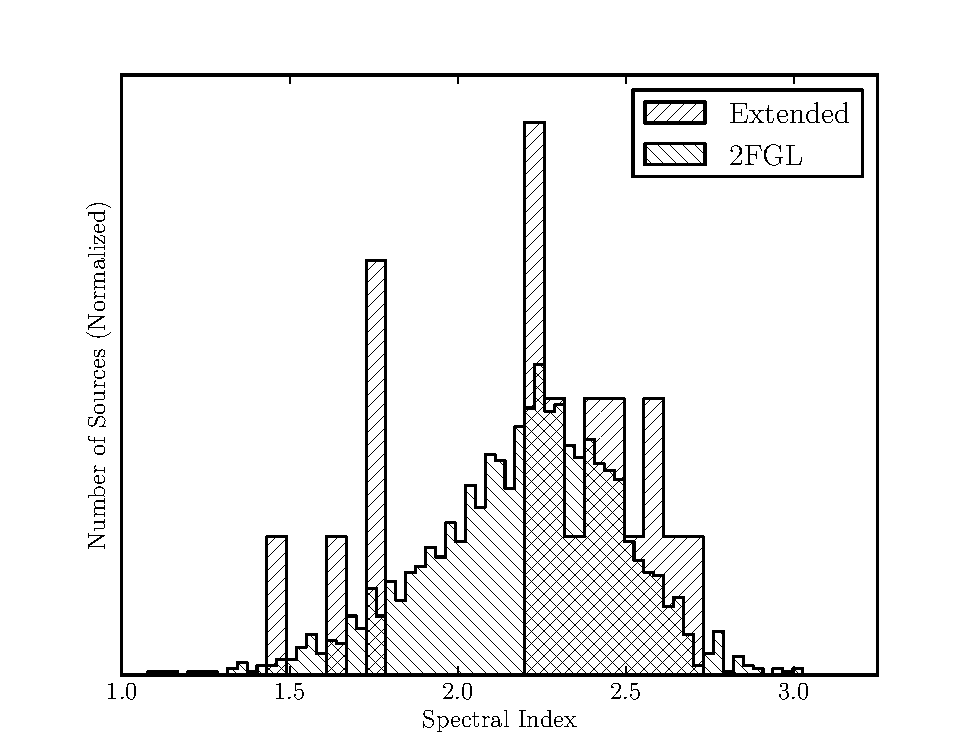
\includegraphics{summary_plots/compare_index_2FGL_bw.pdf}
    \fi
    % plot taken from /u/gl/lande/work/fermi/extended_catalog/2FGL/plots_for_paper/compare_index_2fgl/v3/run.py
    \caption{
    The distribution of spectral indices of the 1873 2FGL sources
    (colored red in the electronic version) and the 21 spatially extended
    sources (colored blue).  The index of Centaurus A is taken from
    \cite{nolan_2012_fermi-large} and the index of Vela X is taken from \cite{abdo_2010c_fermi-large}.
    }\figlabel{compare_index_2FGL}
  \end{figure}



\figref{compare_index_2FGL} compares the spectral indices of LAT
detected extended sources and of all sources in the 2FGL catalog. This, and
\tabref{known_extended_sources} and \tabref{new_ext_srcs_table},
show that the LAT observes a population of hard extended sources
at energies above 10 \gev.  \figref{hess_seds} shows that
the spectra of four of these sources (2FGL\,J1615.0$-$5051,
2FGL\,J1615.2$-$5138, 2FGL\,J1632.4$-$4753c, and 2FGL\,J1837.3$-$0700c)
at \gev energies connects to the spectra of their H.E.S.S. counterparts
at \tev energies. This is also true of Vela Jr., HESS\,J1825$-$137
\citep{grondin_2011_detection-pulsar}, and RX\,J1713.7$-$3946 \citep{abdo_2011a_observations-young}.
It is likely that the \gev and \tev emission from these sources originates
from the same population of high-energy particles.

Many of the \tev-detected extended sources now seen at \gev energies
are currently unidentified and further multiwavelength follow-up
observations will be necessary to understand these particle accelerators.
Extending the spectra of these \tev sources towards lower energies
with LAT observations may help to determine the origin and nature of
the high-energy emission.



